
%% bare_conf.tex
%% V1.4b
%% 2015/08/26
%% by Michael Shell
%% See:
%% http://www.michaelshell.org/
%% for current contact information.
%%
%% This is a skeleton file demonstrating the use of IEEEtran.cls
%% (requires IEEEtran.cls version 1.8b or later) with an IEEE
%% conference paper.
%%
%% Support sites:
%% http://www.michaelshell.org/tex/ieeetran/
%% http://www.ctan.org/pkg/ieeetran
%% and
%% http://www.ieee.org/

%%*************************************************************************
%% Legal Notice:
%% This code is offered as-is without any warranty either expressed or
%% implied; without even the implied warranty of MERCHANTABILITY or
%% FITNESS FOR A PARTICULAR PURPOSE! 
%% User assumes all risk.
%% In no event shall the IEEE or any contributor to this code be liable for
%% any damages or losses, including, but not limited to, incidental,
%% consequential, or any other damages, resulting from the use or misuse
%% of any information contained here.
%%
%% All comments are the opinions of their respective authors and are not
%% necessarily endorsed by the IEEE.
%%
%% This work is distributed under the LaTeX Project Public License (LPPL)
%% ( http://www.latex-project.org/ ) version 1.3, and may be freely used,
%% distributed and modified. A copy of the LPPL, version 1.3, is included
%% in the base LaTeX documentation of all distributions of LaTeX released
%% 2003/12/01 or later.
%% Retain all contribution notices and credits.
%% ** Modified files should be clearly indicated as such, including  **
%% ** renaming them and changing author support contact information. **
%%*************************************************************************


\documentclass[conference]{IEEEtran}
\usepackage{graphicx}
\usepackage{listings}
\usepackage[font=small,labelfont=bf]{caption}


% *** PDF, URL AND HYPERLINK PACKAGES ***
%
%\usepackage{url}

% *** Do not adjust lengths that control margins, column widths, etc. ***
% *** Do not use packages that alter fonts (such as pslatex).         ***
% There should be no need to do such things with IEEEtran.cls V1.6 and later.
% (Unless specifically asked to do so by the journal or conference you plan
% to submit to, of course. )


% correct bad hyphenation here
\hyphenation{op-tical net-works semi-conduc-tor}


\begin{document}
%
% paper title
% Titles are generally capitalized except for words such as a, an, and, as,
% at, but, by, for, in, nor, of, on, or, the, to and up, which are usually
% not capitalized unless they are the first or last word of the title.
% Linebreaks \\ can be used within to get better formatting as desired.
% Do not put math or special symbols in the title.
\title{Parallel Neural Network Framework}


% author names and affiliations
% use a multiple column layout for up to three different
% affiliations
\author{\IEEEauthorblockN{Srajan Garg}
\IEEEauthorblockA{140050017}
\and
\IEEEauthorblockN{Anuj Mittal}
\IEEEauthorblockA{140050024}
\and
\IEEEauthorblockN{Sumith Kulal}
\IEEEauthorblockA{140050081}
\and
\IEEEauthorblockN{Shubham Goel}
\IEEEauthorblockA{140050086}
}

% conference papers do not typically use \thanks and this command
% is locked out in conference mode. If really needed, such as for
% the acknowledgment of grants, issue a \IEEEoverridecommandlockouts
% after \documentclass

% for over three affiliations, or if they all won't fit within the width
% of the page, use this alternative format:
% 
% \author{\IEEEauthorblockN{Srajan Garg\IEEEauthorrefmark{1},
% Anuj Mittal\IEEEauthorrefmark{2},
% Sumith Kulal\IEEEauthorrefmark{3} and
% Shubham Goel\IEEEauthorrefmark{3}}
% \IEEEauthorblockA{\IEEEauthorrefmark{1}140050017}
% \IEEEauthorblockA{\IEEEauthorrefmark{2}140050024}
% \IEEEauthorblockA{\IEEEauthorrefmark{3}140050081}
% \IEEEauthorblockA{\IEEEauthorrefmark{4}140050086}}




% use for special paper notices
%\IEEEspecialpapernotice{(Invited Paper)}




% make the title area
\maketitle

\lstset{
   basicstyle=\fontsize{9}{13}\selectfont\ttfamily
}

% As a general rule, do not put math, special symbols or citations
% in the abstract
\begin{abstract}
Most of the current computer systems use statistical techniques to `learn" with data and progressively improve performance on a specific task. Artificial Neural Networks are one such technique that is extensively used. However computation done in neural networks is intensive and can be vastly benefit from parallel techniques. In this paper, we present a parallel neural network framework. We also attempt to support convolution layer for the neural networks. Most image manipulation tasks use convolution routines. Furthermore, recent work on image manipulation is data-driven and uses such frameworks.  As an example study, we work on a higher level (learning-based) tasks of Optical Character Recognition on the MNIST dataset. The convolution layer in the framework allows us to tackle a wide range of simple (non-learning) image manipulation problems with a single fixed convolution layer (Eg. Blur, Edge Detection etc.).  We have implemented fully connected layers and activation layers in the neural network. All the operations in these layers are inherently parallelizable and we compared the performance of the serial code with parallelized CUDA running on GPU.
\end{abstract}

% no keywords


% For peer review papers, you can put extra information on the cover
% page as needed:
% \ifCLASSOPTIONpeerreview
% \begin{center} \bfseries EDICS Category: 3-BBND \end{center}
% \fi
%
% For peerreview papers, this IEEEtran command inserts a page break and
% creates the second title. It will be ignored for other modes.
\IEEEpeerreviewmaketitle



\section{Introduction}
The size of images is generally huge and a serialized code can be significantly slow when running image manipulation tasks. It becomes further slow when tasks involve machine learning techniques like neural networks which involve processing huge data to train the network. In this project, we show how these processes can run significantly faster with parallelization using GPU. We worked on two problems in this field. 
We compared GPU parallelized to show the speedup gained by GPU parallelization. We also observed that CPU parallelization using OpenMP did not give us a significant reason and try to reason the cause of it.

\section{Neural Network}
To begin with, we write a standalone C++ serial neural network library, and provide a user friendly API. We wanted to give the user the flexibility to choose their own network architecture with simple function calls, just like in popular python libraries like Tensorflow\cite{tensorflow} and PyTorch\cite{pytorch}. We also provide tunable parameters like learning rate and number of training epochs for the network. Next, we parallelize the network using two popular concurrency techniques from different domains. We use OpenMP for CPU parallelization and CUDA for GPU parallelization. We then discuss the approaches used and results obtained.

\subsection{Layers}
The entire network, in essence, is a list of objects of type \textit{Layer}. Each layer has some common operations, and we use pure virtual functions in a base class to specify the operations required. A willing user can even add their own \textit{Layer} by inheriting from the base class and defining the required functions. Each layer has it's own buffer for storing outputs after the forward operation, and also a buffer for storing the gradients that need to be passed to the previous layer. Each layers also stores pointers to the buffers of the previous and next layer to use the data in the forward and backward pass respectively.

The library comes with the following pre-defined layers:
\begin{itemize}
    \item \textbf{Input}: This layer is added to the network by default and acts as a proxy layer for interfacing user supplied data with the network. It has no extraordinary function in the network's learning.
    \item \textbf{Dense}: This layer takes in the number of hidden units as the parameter and adds a fully connected dense layer to the already existing neural network. it borrows the number of the inputs from the existing network, and initializes a weight matrix appropriately.
    \item \textbf{Activation}: This layer adds an activation function on the output of the previous layer. A variety of activation functions have been made available including ReLU and sigmoid.
\end{itemize}

\subsection{Algorithm}
The neural network performs its primary task of learning its tunable parameters when the \textit{train} method is called, which envelopes the three main procedures require for this step in a loop. Apart from these methods, the neural network has some miscellaneous helper functions like \textit{add\textunderscore training \textunderscore data} and \textit{initialize}. The main methods in the network's learning procedure are :
\begin{itemize}
    \item Forward Pass
    \item Error Calculation
    \item BackPropogation
\end{itemize}

Dense Layer Forward:
\begin{equation}
\mathop{out}_{(outF)} = \mathop{Wt}_{(outF X inF)}*\mathop{in}_{(inF)} + \mathop{Bias}_{(outF)}
\end{equation}

Dense Layer Backprop:
\begin{equation}
\frac{\partial E}{\partial in} = \frac{\partial out}{\partial in}*\frac{\partial E}{\partial out} \Rightarrow\quad \delta_{in} = Wt^{T}*\delta_{out}
\end{equation}
\begin{equation}
\frac{\partial E}{\partial Bias} = \frac{\partial out}{\partial Bias}*\frac{\partial E}{\partial out} \Rightarrow\quad \delta_{in} = I*\delta_{out} 
\end{equation}
\begin{equation}
\frac{\partial E}{\partial Wt} = \frac{\partial out}{\partial Wt}*\frac{\partial E}{\partial out} \Rightarrow\quad \delta_{in} = \delta_{out}*in^{T} 
\end{equation}

Activation Layer Forward:
\begin{equation}
out = f(in)
\end{equation}

Activation Layer Backprop:
\begin{equation}
\frac{\partial E}{\partial in} = \frac{\partial out}{\partial in}*\frac{\partial E}{\partial out} \Rightarrow\quad \delta_{in} = f'(\delta_{out})
\end{equation}

\subsection{Parallelization}
Upon careful review of the architecture of our library, we could think of multitudinous ways to parallelize the program. We had to stick to implementing only a subset of these ideas in the best interest of time. We tried the following ways to parallelize our code.
\begin{itemize}
    \item \textbf{CPU}: We can trivially observe that most of the computation involved in the training of the neural network are matrix multiplications. A simple technique to parallelize the entire library was to parallelize this step, which takes up a majority of the program time. (gprof run and see)
    \item \textbf{GPU}: All heavy operations for a neural network with dense layers rely on matrix multiplications. So we decided to accelerate the code by implementing matrix multiplication in the GPU as follows:

\begin{lstlisting}
matmul(float*a, float*b, float*res, ..) 
{
  // Allocate space, Copy data to GPU
  // Call kernel routine
  // Copy data to CPU
}
\end{lstlisting}

However, this code ran much slower than its CPU counterpart. We realized that was because of extensive data transfer between the Host and Device. Every matrix multiplication operation resulted in 6 transfers. Each dense layer's forward + backward pass required 3 matmul operations. For 10000 data points running on a 3 layer network, this meant 54000 transfers per epoch!

As a remedy, we decided to first move all data to GPU, then operate on it. So ALL operations had to be implemented in CUDA. To facilitate book-keeping and easy handling, we wrapped all data pointers (in both Host and Device) by a common class `Tensor' with the following members:

\begin{lstlisting}
class Tensor {
  float* data
  bool is_cuda
  int ndims
  float shape[NDIMS_MAX]
}
\end{lstlisting}

All data was moved to GPU in the very beginning and each operation on Tensors was implemented for both CPU (C++) and GPU (CUDA). Here is what the matmul operation looked like:

\begin{lstlisting}
matmul(Tensor a, Tensor b, Tensor res,..) 
{
  if (is_cuda)  // CUDA matmul routine
    Run matmul_cuda( ... )
  else  // CPU matmul routine
    Run matmul_cpu( ... )
}
\end{lstlisting}

Other Tensor operations that had to be implemented in CUDA include addition, subtraction, and multiplication for scalar and matrix. A complete list has been added in the appendix. This gave considerable speedups over the CPU code, as expected.
\end{itemize}


\subsection{Solving a Real World Problem}
It is time to put our library to the test! We went ahead with a problem which is relatively simple but still maintains practical relevance in the real world. The handwritten digit recognition problem seems like a good fit, and achieves decent accuracy on relatively simple dense networks.
We used the classic MNIST dataset\cite{mnist} for our experiments and benchmarking our neural network speeds. The following architecture is used for the task in hand. This also sheds light on how easy it is to setup an architecture in our framework.

\begin{lstlisting}
NN nn(784);
nn.add_layer(new Dense(800));
nn.add_layer(new 
    Activation(Activations::SIGMOID, 800));
nn.add_layer(new Dense(10));
nn.add_layer(new 
    Activation(Activations::SIGMOID, 10));

nn.initialize(0.01, Errors::CROSSENTROPY);
\end{lstlisting}

 \\

\section{Image Manipulation by fixed Convolution}
In image processing, several objectives like blurring, sharpening, edge detection can be achieved by a convolution between a convolution matrix (also known as kernel or mask) and an image. In a convolution, we sweep the kernel over the image and combine pixels and kernel values with multiplication, then summarize the results with addition.  To help us with image utilities like read/write of images, we use the CImg library\cite{CImg}.

 \\
\subsection{Algorithm}
Convolution with some specific kernels leads to very interesting results. For example, if we use a kernel with all elements as 1, we get a blurring effect and this is known as box blur. As a part of our evaluation, we have implemented kernels that perform box blur, gaussian blur, edge detection, sharpening and embossing.

\begin{frame}
\frametitle{Convolution over an image}
  \lstset{language=C++}
\begin{lstlisting}
for x = 0 to image_x 
  for y = 0 to image_y
    for z = 0 to image_z
      perform single pixel convolution
\end{lstlisting}
\end{frame}


\begin{frame}
\frametitle{Single Pixel Convolution}
  \lstset{language=C++}
\begin{lstlisting}
result = 0
for x = 0 to kernel_x
  for y = 0 to kernel_y
    if image_pixel exists at x, y 
      result += kernel_value * pixel_value
output_pixel = result
\end{lstlisting}
\end{frame}

\vspace{-20pt}

\subsection{Parallelization}
We observe that computation at every pixel is independent of the computation at other pixels. We also observe that multiplication in a single pixel computation can be parallelized as long as we ensure that all the multiplication is completed before we summarize and do the addition. \\
\subsubsection{GPU Parallelization}
We parallelize the convolution using CUDA. We adjust the number of blocks and number of threads such that a single pixel computation is done by one block and single multiplication in this computation is done by one thread. We ensure that all threads terminate by using \textunderscore \textunderscore syncthreads() before the final addition.
\subsubsection{CPU Parallelization}
We used OpenMP to achieve CPU parallelization through multiple threads. Apart from parallelizing the convolution, we also parallelized the generation of kernels which was not adequeate to parallelize on CUDA due to its relatively small size.

\vspace{-10pt}
\section{Results}
We ran our framework on the MNIST dataset as mentioned before. We present the time taken by the serial code, OpenMP code with different number of threads and CUDA code at various training epoch levels. We also present the time taken for applying effects using kernel on a sample image along with the output images.




\afterpage{%
  \noindent \begin{minipage}{2\columnwidth}
 \begin{center}
 \begin{tabular}{|c|c c c c c|c|} 
 \hline
 Epoch & Serial & 2 thr & 4 thr & 8 thr & CUDA & Speedup(CUDA) \\ [0.5ex] 
 \hline\hline
1 & 19.88 & 11.06 & 5.51 & 7.15 & 5.28 & 3.77 \\
5 & 104.51 & 60.64 & 34.80 & 37.16 & 26.33 & 3.97 \\
10 & 210.94 & 126.06 & 72.04 & 73.92 & 52.66 & 4.01 \\ [1ex] 
 \hline
\end{tabular}
\end{center}
\begin{center}
 \begin{tabular}[!b]{|c|c c c c c|c|} 
 \hline
 Effect & Serial & 2 thr & 4 thr & 8 thr & CUDA & Speedup(CUDA) \\ [0.5ex] 
 \hline\hline
Box Blur & 140.46 & 74.24 & 48.00 & 45.73 & 6.53 & 21.50 \\
Gauss Blur & 288.50 & 180.08 & 99.60 & 100.72 & 11.43 & 25.24 \\
Edge Detection & 34.22 & 23.98 & 12.51 & 11.34 & 3.79 & 9.03 \\
High Pass filter & 17.77 & 12.96 & 7.16 & 6.46 & 2.91 & 6.11 \\
Sharpen & 17.85 & 12.95 & 6.95 & 7.32 & 2.75 & 6.50 \\
Emboss & 17.44 & 12.27 & 6.29 & 7.01 & 2.13 & 8.17 \\
Total & 517.27 & 317.23 & 181.13 & 179.18 & 31.19 & 16.59 \\ [1ex] 
 \hline
\end{tabular}
\end{center}
\end{minipage}
}


% \hspace{-30pt}
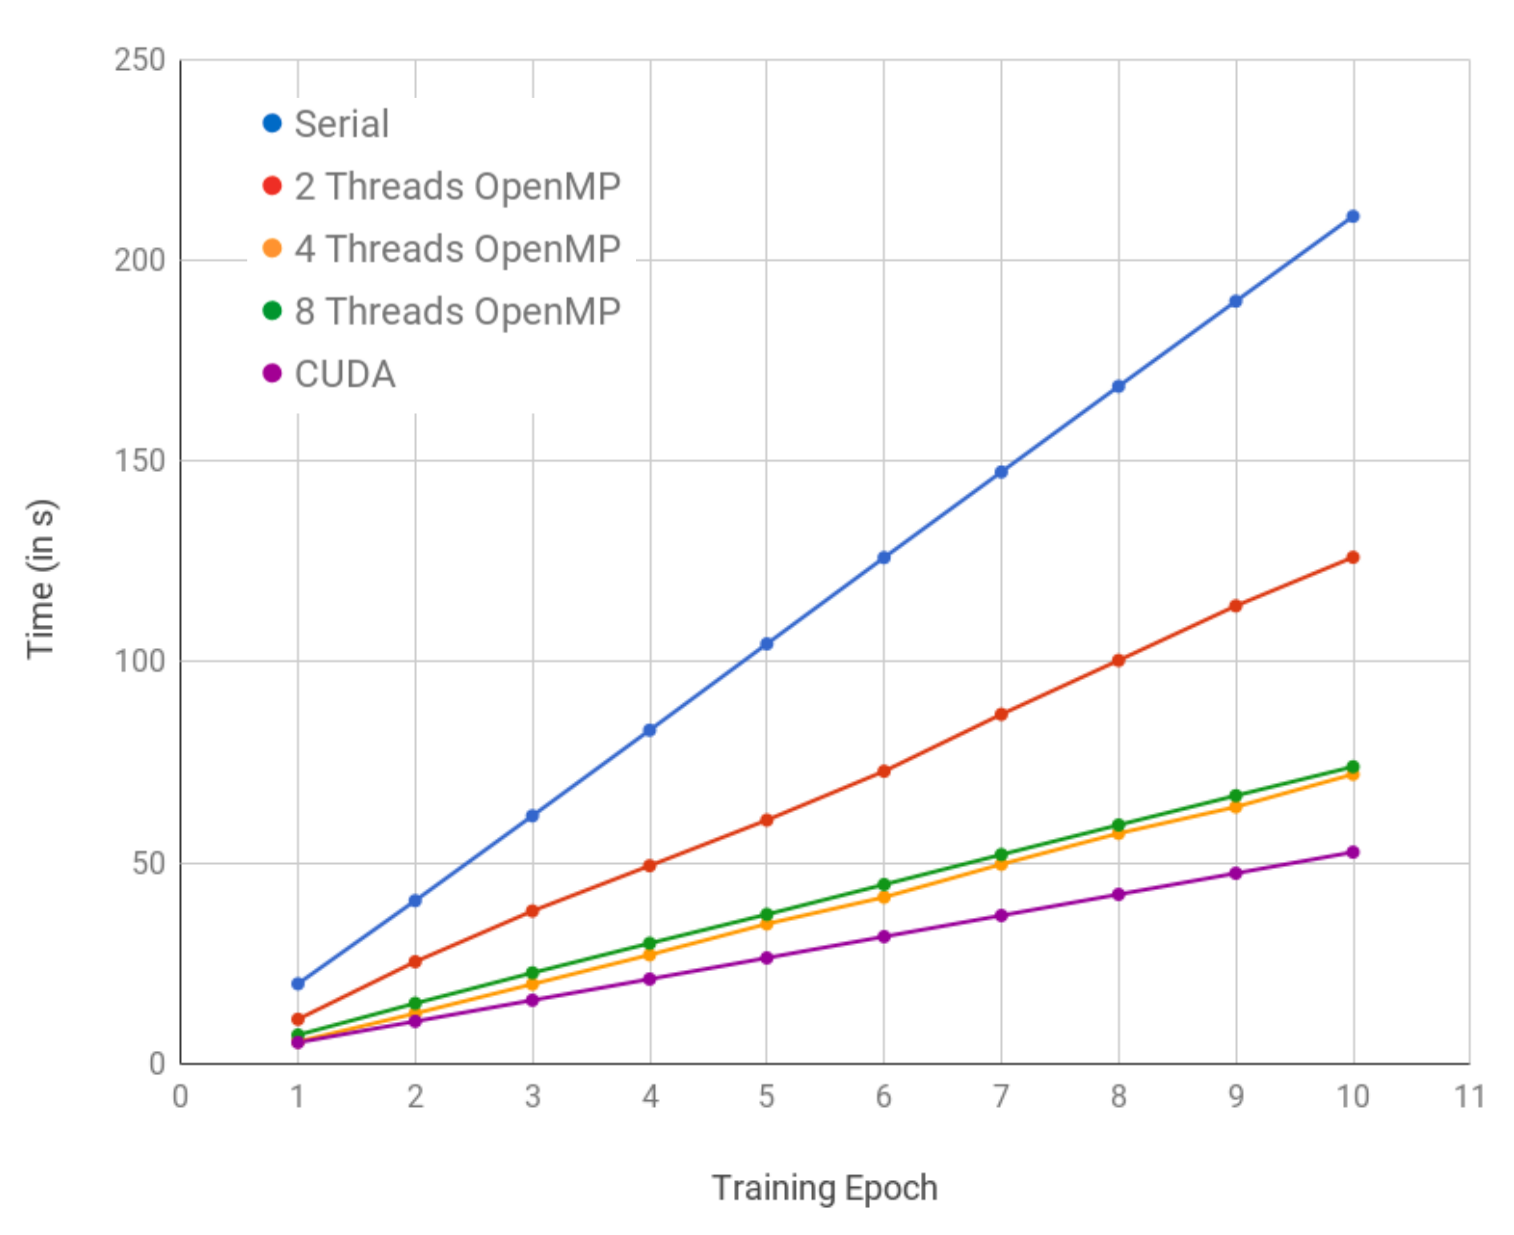
\includegraphics[width=\linewidth]{images/nn_graph.png}
\captionof{figure}{Neural Network Runtime}

% \hspace{-30pt}
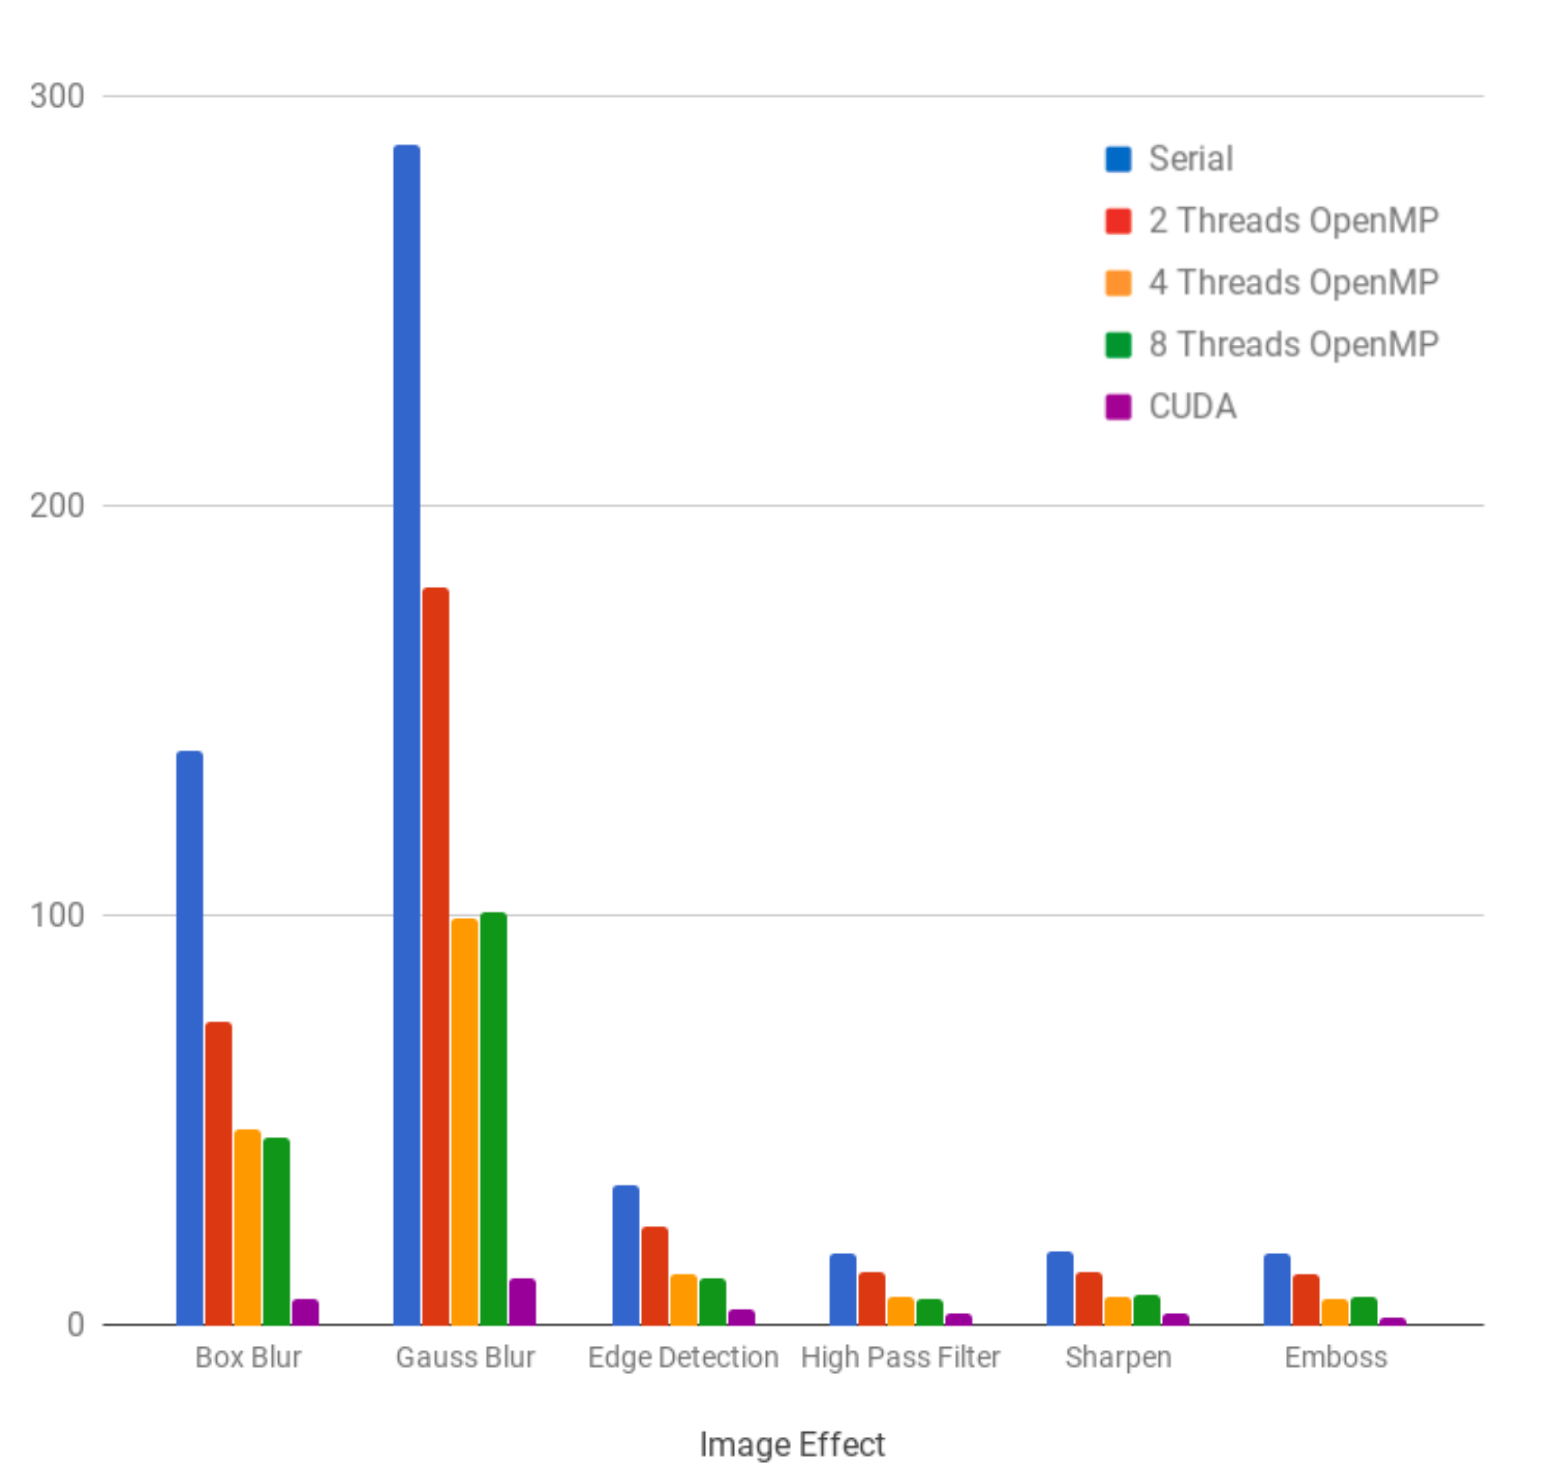
\includegraphics[width=\linewidth]{images/conv_graph.png}
\captionof{figure}{Convolution Runtime}

\newpage

\includegraphics[width=0.48\textwidth]{images/infinity-war.jpg}
\captionof{figure}{Original Image}

% \includegraphics[width=0.48\textwidth]{images/blur-box.jpg}
% \captionof{figure}{Blur Box}

\includegraphics[width=0.48\textwidth]{images/blur-gauss.jpg}
\captionof{figure}{Blur Gauss}

\includegraphics[width=0.48\textwidth]{images/edge.jpg}
\captionof{figure}{Edge Detection}

\includegraphics[width=0.48\textwidth]{images/emboss.jpg}
\captionof{figure}{Emboss}

\includegraphics[width=0.48\textwidth]{images/highpass.jpg}
\captionof{figure}{Highpass Filter}

\includegraphics[width=0.48\textwidth]{images/sharpen.jpg}
\captionof{figure}{Sharpen}


% An example of a floating figure using the graphicx package.
% Note that \label must occur AFTER (or within) \caption.
% For figures, \caption should occur after the \includegraphics.
% Note that IEEEtran v1.7 and later has special internal code that
% is designed to preserve the operation of \label within \caption
% even when the captionsoff option is in effect. However, because
% of issues like this, it may be the safest practice to put all your
% \label just after \caption rather than within \caption{}.
%
% Reminder: the "draftcls" or "draftclsnofoot", not "draft", class
% option should be used if it is desired that the figures are to be
% displayed while in draft mode.
%
%\begin{figure}[!t]
%\centering
%\includegraphics[width=2.5in]{myfigure}
% where an .eps filename suffix will be assumed under latex, 
% and a .pdf suffix will be assumed for pdflatex; or what has been declared
% via \DeclareGraphicsExtensions.
%\caption{Simulation results for the network.}
%\label{fig_sim}
%\end{figure}

% Note that the IEEE typically puts floats only at the top, even when this
% results in a large percentage of a column being occupied by floats.


% An example of a double column floating figure using two subfigures.
% (The subfig.sty package must be loaded for this to work.)
% The subfigure \label commands are set within each subfloat command,
% and the \label for the overall figure must come after \caption.
% \hfil is used as a separator to get equal spacing.
% Watch out that the combined width of all the subfigures on a 
% line do not exceed the text width or a line break will occur.
%
%\begin{figure*}[!t]
%\centering
%\subfloat[Case I]{\includegraphics[width=2.5in]{box}%
%\label{fig_first_case}}
%\hfil
%\subfloat[Case II]{\includegraphics[width=2.5in]{box}%
%\label{fig_second_case}}
%\caption{Simulation results for the network.}
%\label{fig_sim}
%\end{figure*}
%
% Note that often IEEE papers with subfigures do not employ subfigure
% captions (using the optional argument to \subfloat[]), but instead will
% reference/describe all of them (a), (b), etc., within the main caption.
% Be aware that for subfig.sty to generate the (a), (b), etc., subfigure
% labels, the optional argument to \subfloat must be present. If a
% subcaption is not desired, just leave its contents blank,
% e.g., \subfloat[].


% An example of a floating table. Note that, for IEEE style tables, the
% \caption command should come BEFORE the table and, given that table
% captions serve much like titles, are usually capitalized except for words
% such as a, an, and, as, at, but, by, for, in, nor, of, on, or, the, to
% and up, which are usually not capitalized unless they are the first or
% last word of the caption. Table text will default to \footnotesize as
% the IEEE normally uses this smaller font for tables.
% The \label must come after \caption as always.
%
%\begin{table}[!t]
%% increase table row spacing, adjust to taste
%\renewcommand{\arraystretch}{1.3}
% if using array.sty, it might be a good idea to tweak the value of
% \extrarowheight as needed to properly center the text within the cells
%\caption{An Example of a Table}
%\label{table_example}
%\centering
%% Some packages, such as MDW tools, offer better commands for making tables
%% than the plain LaTeX2e tabular which is used here.
%\begin{tabular}{|c||c|}
%\hline
%One & Two\\
%\hline
%Three & Four\\
%\hline
%\end{tabular}
%\end{table}


% Note that the IEEE does not put floats in the very first column
% - or typically anywhere on the first page for that matter. Also,
% in-text middle ("here") positioning is typically not used, but it
% is allowed and encouraged for Computer Society conferences (but
% not Computer Society journals). Most IEEE journals/conferences use
% top floats exclusively. 
% Note that, LaTeX2e, unlike IEEE journals/conferences, places
% footnotes above bottom floats. This can be corrected via the
% \fnbelowfloat command of the stfloats package.


\section{Conclusion}
In this paper, we present a small but feature packed neural network framework. This framework was built from scratch and achieves high performance leveraging parallelization from CUDA. We also implemented and evaluated our convolution on a variety of images, producing good results in a small time.

\section{Future Work}
A natural immediate extension to our framework would be implementing backprop for our convolution layer. We can also make our convolution and matrix multiplication routines much faster using cache locality. This would open possibilities for our framework to train machine learning models on images. Additionally, there are tons of neural network features that can be added to this framework to bring it closer to full fledged frameworks like PyTorch and Tensorflow. Support for new layers, new activation layers, etc., can be added with no end in sight. 





% trigger a \newpage just before the given reference
% number - used to balance the columns on the last page
% adjust value as needed - may need to be readjusted if
% the document is modified later
%\IEEEtriggeratref{8}
% The "triggered" command can be changed if desired:
%\IEEEtriggercmd{\enlargethispage{-5in}}

% references section

% can use a bibliography generated by BibTeX as a .bbl file
% BibTeX documentation can be easily obtained at:
% http://mirror.ctan.org/biblio/bibtex/contrib/doc/
% The IEEEtran BibTeX style support page is at:
% http://www.michaelshell.org/tex/ieeetran/bibtex/
%\bibliographystyle{IEEEtran}
% argument is your BibTeX string definitions and bibliography database(s)
%\bibliography{IEEEabrv,../bib/paper}
%
% <OR> manually copy in the resultant .bbl file
% set second argument of \begin to the number of references
% (used to reserve space for the reference number labels box)

\bibliographystyle{IEEEtran}
\bibliography{ref}




% that's all folks
\end{document}


